\documentclass[letterpaper, 11pt]{article}
\usepackage[utf8]{inputenc}
\usepackage[letterpaper, portrait, margin=1in]{geometry}
\usepackage{pgfplots}
\pgfplotsset{width=10cm,compat=1.9}
\usepackage{hyperref}
\usepackage{textcomp}
\usepackage{siunitx}
\usepackage{amsmath}
\usepackage{cancel}
\usepackage{tikz}
\usepackage{tikzit}
\usepackage{everysel}
\usepackage{ragged2e}
\usepackage{mathdots}
\usepackage{yhmath}
\usepackage{color}
\usepackage{array}
\usepackage{multirow}
\usepackage{amssymb}
\usepackage{gensymb}
\usepackage{tabularx}
\usepackage{booktabs}
\usepackage{listings}
\usepackage{xcolor}
\usepackage{enumitem}
\usetikzlibrary{fadings}
\usetikzlibrary{patterns}
\usetikzlibrary{shadows.blur}
\hypersetup{
    colorlinks=true,
    linkcolor=black,
    filecolor=black,      
    urlcolor=blue,
}

\input{main.tikzstyles}

\definecolor{codegreen}{rgb}{0,0.6,0}
\definecolor{codegray}{rgb}{0.5,0.5,0.5}
\definecolor{codepurple}{rgb}{0.58,0,0.82}
\definecolor{backcolour}{rgb}{0.95,0.95,0.92}

\lstdefinestyle{mystyle}{
    backgroundcolor=\color{backcolour},   
    commentstyle=\color{codegreen},
    keywordstyle=\color{magenta},
    numberstyle=\tiny\color{codegray},
    stringstyle=\color{codepurple},
    basicstyle=\ttfamily\footnotesize,
    breakatwhitespace=false,         
    breaklines=true,                 
    captionpos=b,                    
    keepspaces=true,                 
    numbers=left,                    
    numbersep=5pt,                  
    showspaces=false,                
    showstringspaces=false,
    showtabs=false,                  
    tabsize=2
}

\lstset{style=mystyle}

\title{COMSC-200 \\ Lab 3}
\author{Ryan Jacoby}
\date{13 September 2020}
\begin{document}

\maketitle

\section{Base and Derived Classes}

\begin{enumerate}[label=\alph*.]
 \item Base class: Employee \\ Derived class: Manager
 \item Base class: Polygon \\ Derived class: Triangle
 \item Base class: Student \\ Derived class: GraduateStudent
 \item Base class: Person \\ Derived class: Student
 \item Base class: Employee \\ Derived class: Professor
 \item Base class: BankAccount \\ Derived class: CheckingAccount
 \item Base class: Vehicle \\ Derived class: Car
 \item Base class: Vehicle \\ Derived class: Minivan
 \item Base class: Car \\ Derived class: Minivan
 \item Base class: Vehicle \\ Derived class: Truck
\end{enumerate}

\section{Inheritance Relationships}

\ctikzfig{r10.3}

\section{Program}

What does the following program print?

\begin{lstlisting}[language=C++]
#include<iostream>

using namespace std;

class B {
public:
    void print(int n) const;
};

void B::print(int n) const {
    cout << n << endl;
}

class D : public B {
public:
    void print(int n) const;
};

void D::print(int n) const {
    if (n <= 1) { B::print(n); }
    else if (n % 2 == 0) { print(n / 2); }
    else { print(3 * n + 1); }
}

int main() {
    D d;
    d.print(3);
    return 0;
}
\end{lstlisting}

This program outputs 1.

\pagebreak
\section{Person, Student, and Instructor Classes}

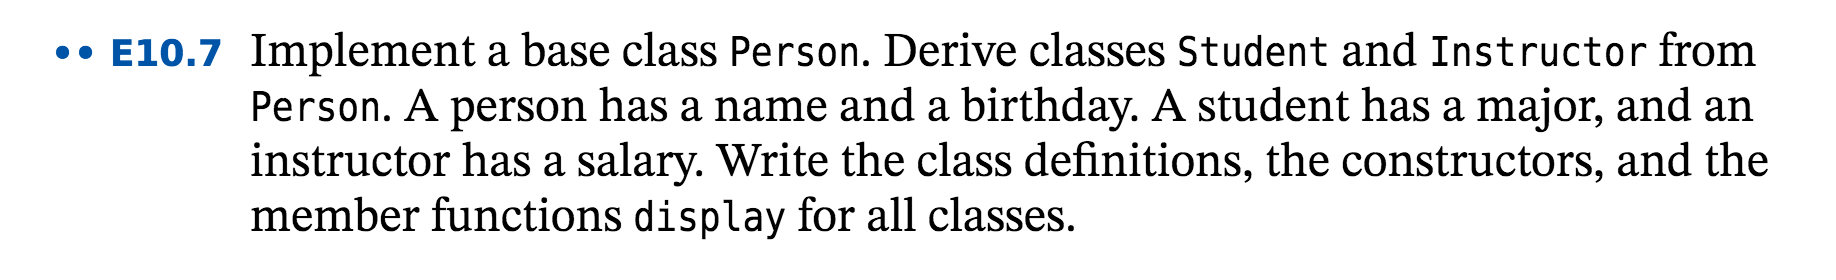
\includegraphics[scale=0.5]{person.png}

\begin{lstlisting}[language=C++, caption=main.cpp]
// Ryan Jacoby

#include<iostream>

#include"Person.h"
#include"Student.h"
#include"Instructor.h"

using namespace std;

int main() {
    Person p = Person("Ryan");
    Student s = Student("Fred", "", "CS");
    Instructor i = Instructor("Ethan", "", 5);

    p.display();
    cout << '\n';
    s.display();
    cout << '\n';
    i.display();

    return 0;
}
\end{lstlisting}

\begin{lstlisting}[language=C++, caption=Person.h]
// Ryan Jacoby

#ifndef Person_h
#define Person_h

#include<string>

using namespace std;

class Person {
private:
    string name;
    string birthday;
public:
    Person();
    Person(string name);
    Person(string name, string birthday);

    string getName() { return this->name; }
    string getBirthday() { return this->birthday; }

    void setName(string name) { this->name = name; }
    void setBirthday(string birthday) { this->birthday = birthday; }

    void display();
};

#endif
\end{lstlisting}

\begin{lstlisting}[language=C++, caption=PersonImp.cpp]
// Ryan Jacoby

#include<iostream>
#include<string>

#include"Person.h"

using namespace std;

Person::Person() {
    this->name = "";
    this->birthday = "";
}

Person::Person(string name) {
    this->name = name;
    this->birthday = "";
}

Person::Person(string name, string birthday) {
    this->name = name;
    this->birthday = birthday;
}

void Person::display() {
    cout << "Name: " << this->name << '\n'
         << "Birthday: " << this->birthday << '\n';
}
\end{lstlisting}

\begin{lstlisting}[language=C++, caption=Student.h]
// Ryan Jacoby

#ifndef Student_h
#define Student_h

#include<string>

using namespace std;

class Student : public Person{
private:
    string major;
public:
    Student() :Person() {}
    Student(string name) :Person(name) {}
    Student(string name, string birthday) :Person(name, birthday) {}
    Student(string name, string birthday, string major);

    string getMajor() { return this->major; }

    void setMajor(string major) { this->major = major; }

    void display();
};

#endif
\end{lstlisting}

\begin{lstlisting}[language=C++, caption=StudentImp.cpp]
// Ryan Jacoby

#include<iostream>
#include<string>

#include"Person.h"
#include"Student.h"

using namespace std;

Student::Student(string name, string birthday, string major) :Person(name, birthday) {
    this->major = major;
}

void Student::display() {
    Person::display();
    cout << "Major: " << this->major << '\n';
}
\end{lstlisting}

\begin{lstlisting}[language=C++, caption=Instructor.h]
// Ryan Jacoby

#ifndef Instructor_h
#define Instructor_h

#include<string>

using namespace std;

class Instructor : public Person{
private:
    int salary;
public:
    Instructor() :Person() {}
    Instructor(string name) :Person(name) {}
    Instructor(string name, string birthday) :Person(name, birthday) {}
    Instructor(string name, string birthday, int salary);

    int getSalary() { return this->salary; }

    void setMajor(int salary) { this->salary = salary; }

    void display();
};

#endif
\end{lstlisting}

\begin{lstlisting}[language=C++, caption=InstructorImp.cpp]
// Ryan Jacoby

#include<iostream>
#include<string>

#include"Person.h"
#include"Instructor.h"

using namespace std;

Instructor::Instructor(string name, string birthday, int salary) :Person(name, birthday) {
    this->salary = salary;
}

void Instructor::display() {
    Person::display();
    cout << "Salary: " << this->salary << '\n';
}
\end{lstlisting}

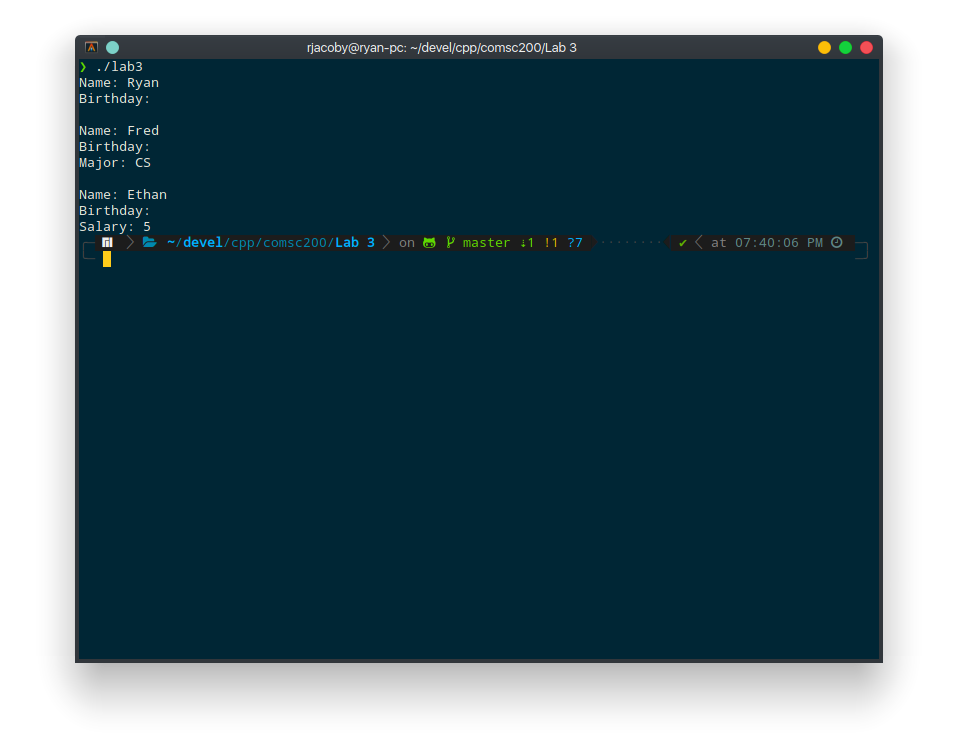
\includegraphics[scale=0.5]{person_run.png}

\section{Clock}

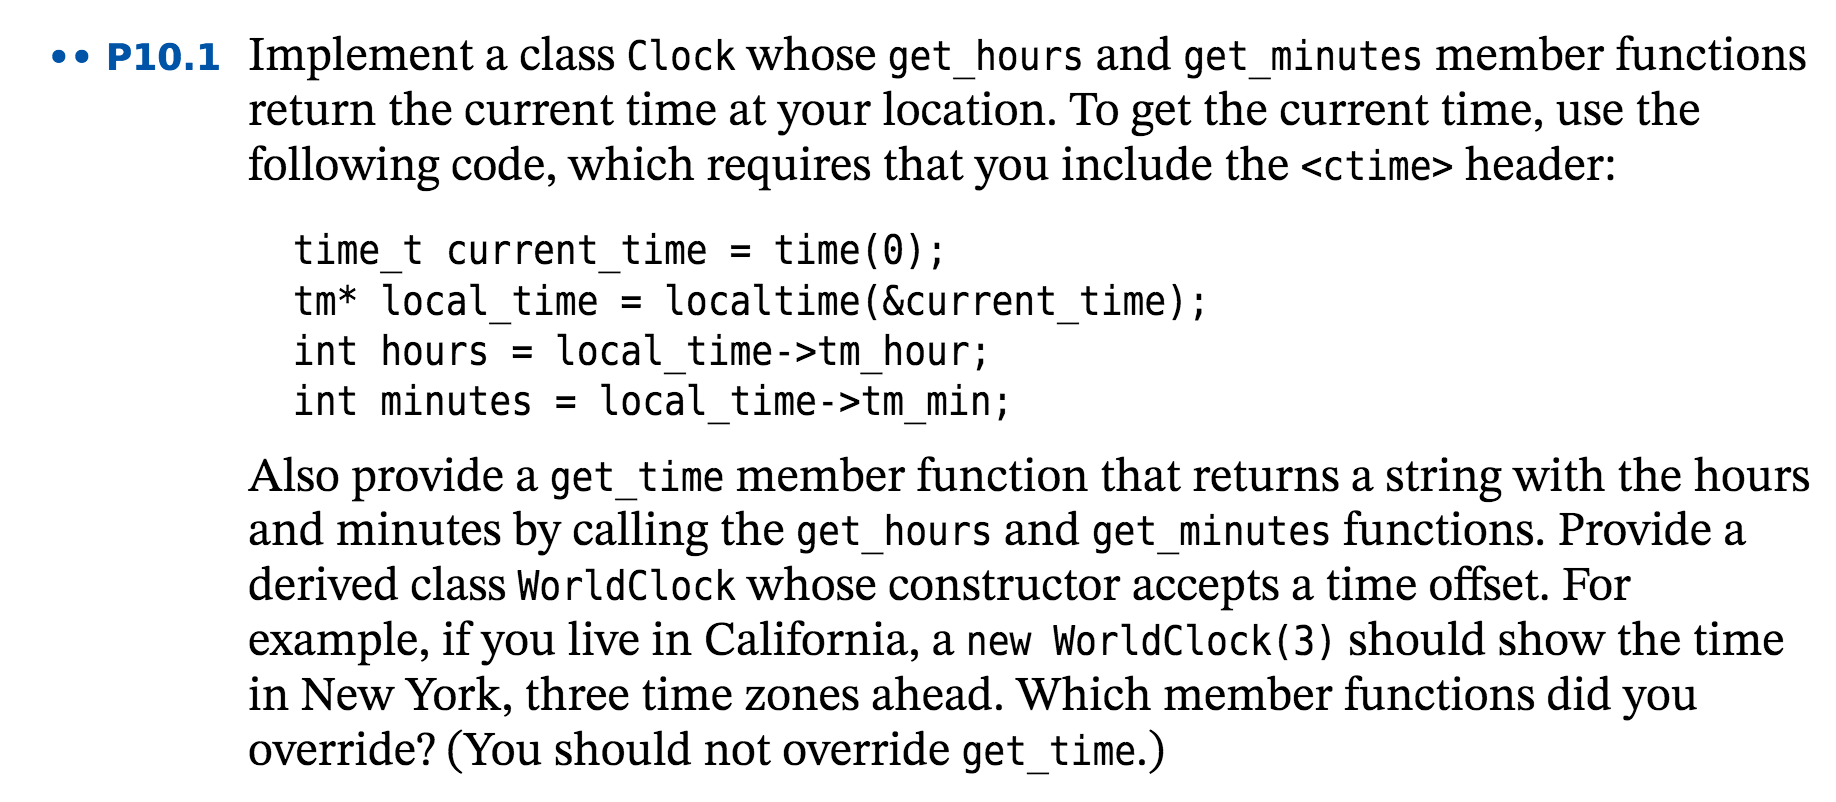
\includegraphics[scale=0.5]{clock.png}

The get\_hours() function is overrided.  I made get\_minutes() virtual so other classes could overwride it for time zones with offset minutes.

\begin{lstlisting}[language=C++, caption=main.cpp]
// Ryan Jacoby

#include<iostream>

#include"Clock.h"
#include"WorldClock.h"

using namespace std;

int main() {
    Clock c = Clock();
    WorldClock wc = WorldClock(3);

    cout << "San Francisco: " << c.get_time() << '\n';
    cout << "New York: " << wc.get_time() << '\n';

    return 0;
}
\end{lstlisting}

\begin{lstlisting}[language=C++, caption=Clock.h]
// Ryan Jacoby

#ifndef Clock_h
#define Clock_h

#include<string>

using namespace std;

class Clock {
protected:
    time_t current_time;
    tm* local_time;
public:
    Clock();

    virtual int get_hours();
    virtual int get_minutes();
    string get_time();
};

#endif
\end{lstlisting}

\begin{lstlisting}[language=C++, caption=ClockImp.cpp]
// Ryan Jacoby

#include<ctime>
#include<string>

#include"Clock.h"

Clock::Clock() {
    this->current_time = time(0);
    this->local_time = localtime(&current_time);
}

int Clock::get_hours() {
    return this->local_time->tm_hour;
}

int Clock::get_minutes() {
    return this->local_time->tm_min;
}

string Clock::get_time() {
    return to_string(get_hours()) + ":" + to_string(get_minutes());
}
\end{lstlisting}

\begin{lstlisting}[language=C++, caption=WorldClock.h]
// Ryan Jacoby

#ifndef WorldClock_h
#define WorldClock_h

using namespace std;

class WorldClock : public Clock {
private:
    int offset;
public:
    WorldClock();
    WorldClock(int offset);

    int get_hours();
};

#endif
\end{lstlisting}

\begin{lstlisting}[language=C++, caption=WorldClockImp.cpp]
// Ryan Jacoby

#include<string>

#include"Clock.h"
#include"WorldClock.h"

WorldClock::WorldClock() :Clock() {
    this->offset = 0;
}

WorldClock::WorldClock(int offset) :Clock() {
    this->offset = offset;
}

int WorldClock::get_hours() {
    return this->local_time->tm_hour + this->offset;
}
\end{lstlisting}

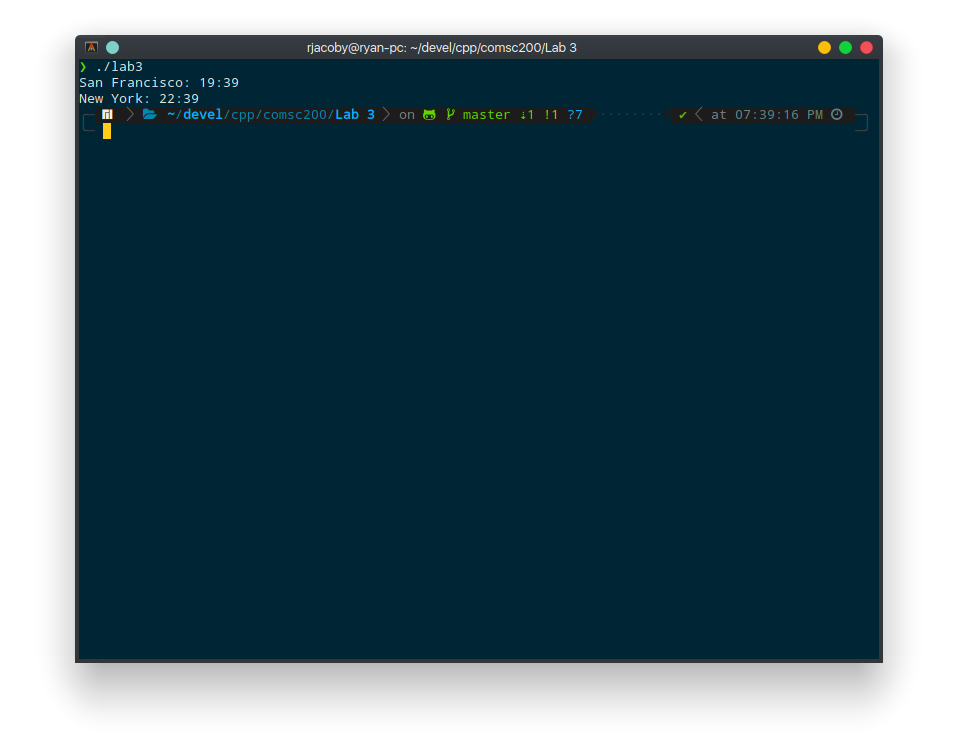
\includegraphics[scale=0.5]{clock_run.png}

\end{document}
